\documentclass[dvipsnames,svgnames]{beamer}
\mode<presentation>
{
\usetheme{PaloAlto}
\usecolortheme{dolphin}
\setbeamercovered{transparent}
}

\usepackage{pdfpages}
\usepackage{stmaryrd}
\usepackage{multicol}
\usepackage[english]{babel}
\usepackage{units}
\usepackage{tikz}
\usepackage{graphicx}
\usepackage{array}
\usepackage{enumerate}
\usepackage{hyperref}
\usepackage[utf8]{inputenc}
\usepackage[brazilian,hyperpageref]{backref}

\title[VLC]{Comunicação Óptica por Luz Visível}
\author{Vilmey Francisco Romano Filho}%\\\texttt{ vilmeyr@gmail.com}}

\institute[Universities of]
{
Universidade de Brasília – UnB\\
Faculdade do Gama – FGA\\
Engenharia Eletrônica\\
}

\date{\today}



\begin{document}

\begin{frame}
\maketitle
\end{frame}

\section{Introdução a Comunicação Óptica sem Fio}

\begin{frame}{Características}

\begin{itemize}

\item Não guiada;
\pause
\item Não regulamentada;
\pause
\item Uso em áreas restritas;
\pause
\item Faixa de luz vizível, infravermelho ou ultravioleta;
\pause
\item Reduzida emissão de interfêrencia eletromagnética.
\end{itemize}

\begin{figure}[!htb]
	\centering
		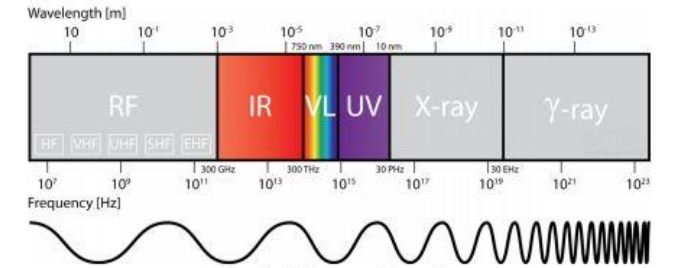
\includegraphics[width=7cm]{figuras/faixas}
		\caption{Faixas utilizadas no OWC.}
		\label{fig:Faixas utilizadas no OWC}
\end{figure}

\end{frame}


%\subsection{Evolução da Comunicação Óptica}
\begin{frame}{Evolução da Comunicação Óptica}

\begin{figure}[!htb]
	\centering
		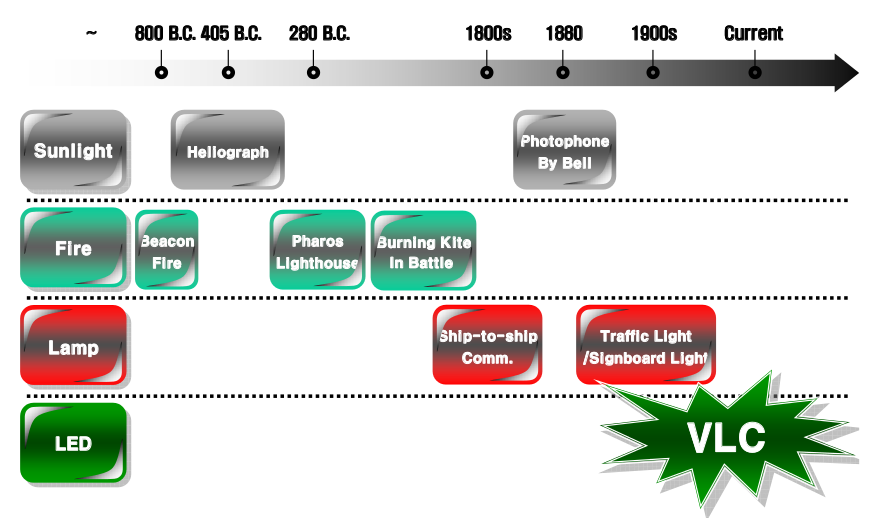
\includegraphics[width=7cm]{figuras/evolucao}
		\caption{Comunicação Óptica desde os primórdios}
		\label{fig:Primordios}
\end{figure}

\end{frame}

%\subsection{Classificação das OWC}
\begin{frame}{Classificação das OWC}

O OWC contém as faixas de luz visíveis, infravermelho e ultravioleta.\\
Neste trabalho será abordada a tacnologia VLC.

\begin{figure}[!htb]
	\centering
		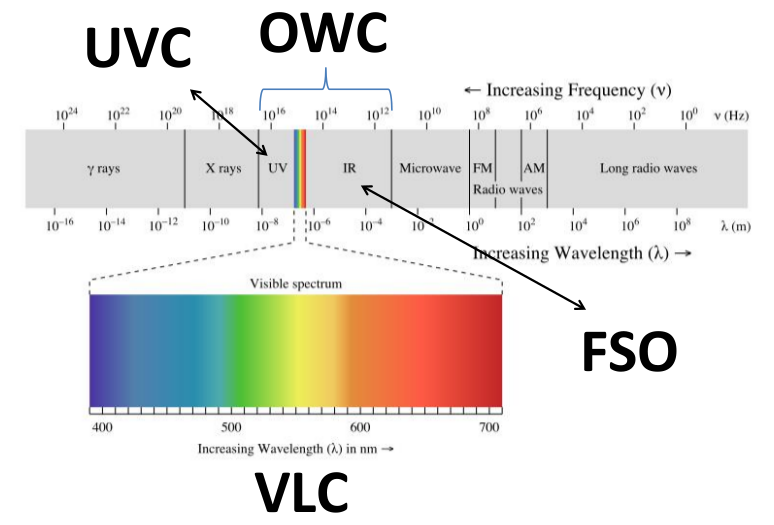
\includegraphics[width=7cm]{figuras/classificacao}
		\caption{Divisão dos espectros ópticos.}
		\label{fig:Espectros opticos}
\end{figure}

\end{frame}


%\subsection{Classificações de Alcance}
\begin{frame}{Classificações de Alcance}

A comunicação óptica pode ser utilizada desde pequenas distâncias como dentro de um circuito, até longas distâncias ex. Lua-Terra.

\begin{figure}[!htb]
	\centering
		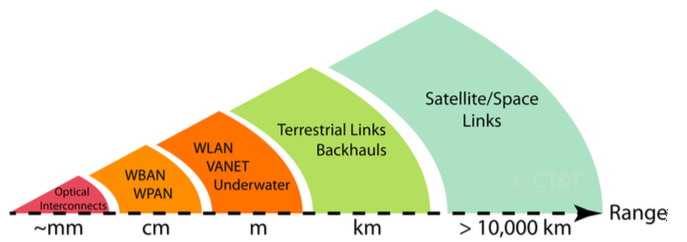
\includegraphics[width=7cm]{figuras/alcance}
		\caption{Divisão de alcance e tipos de transmissão óptica.}
		\label{fig:Classificacao}
\end{figure}

\end{frame}

%\subsubsection{Ultra-Short Range}
\begin{frame}{Ultra-Short Range}

\begin{itemize}
	\item Substituição do cobre;
	\pause
	\item Transmissão Inter/Intra chip;
	\pause
	\item Baixa latência;
	\pause
	\item Alta taxa de transmissão de dados.
\end{itemize}


\begin{figure}[!htb]
	\centering
		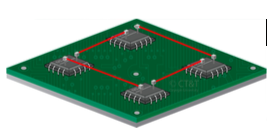
\includegraphics[width=7cm]{figuras/ultra-short}
		\caption{Transferencia de dados entre CI`s.}
		\label{fig:ultra-short}
\end{figure}

\end{frame}


%\subsubsection{Short-Range}
\begin{frame}{Short-Range}

\begin{itemize}
	\item Aplicações hospitalares;
	\pause
	\item Áreas restritas;
	\pause
	\item Bases aéreas;
	\pause	
	\item Aviões.
\end{itemize}

\begin{figure}[!htb]
	\centering
		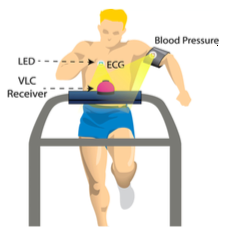
\includegraphics[width=4cm]{figuras/short}
		\caption{Dados de teste de esforço cardíaco enviados via luz.}
		\label{fig:ultra-short}
\end{figure}


\end{frame}

\subsubsection{Medium-Range}
\begin{frame}{Médio Alcance}

Será o foco de aplicação deste trabalho a área de alcançe médio.

\begin{itemize}

	\item Opera na ordem de metros;
	\pause
	\item Pode substituir o Wi-Fi;
	\pause
	\item Longa vida (LED e Fotodiodo);
	\pause
	\item Tolerância a umidade;
	\pause
	\item Menor consumo de energia elétrica em relação ao RF.
	
\end{itemize}

\begin{figure}[!htb]
	\centering
		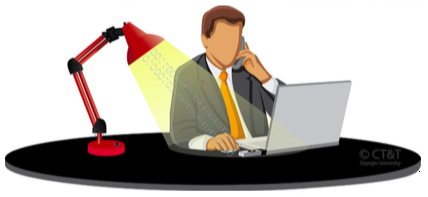
\includegraphics[width=4cm]{figuras/medio1}
		\caption{Luminária utilizada como ponto de acesso.}
		\label{fig:alcance medio}
\end{figure}


\end{frame}

\subsection{OWC vs Rádio}
\begin{frame}{OWC vs Rádio}

Motivos que incentivam a ampliação da tecnologia óptica sem fio.
\begin{figure}[!htb]
	\centering
		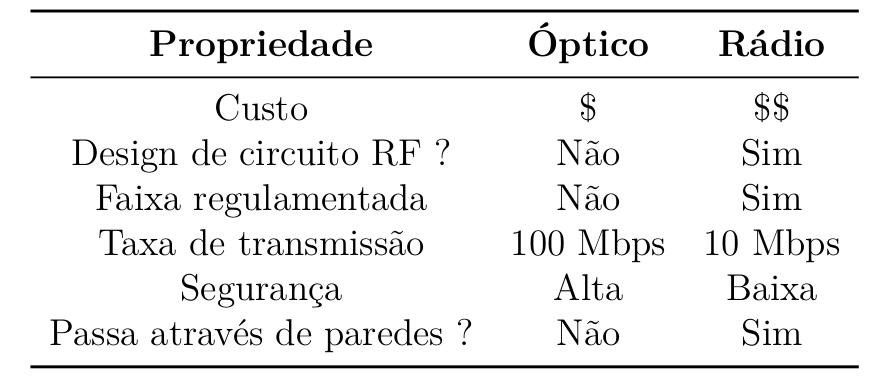
\includegraphics[width=7cm]{figuras/vlc_radio}
		\caption{Benefícios da transmissão óptica.}
		\label{fig:alcance medio}
\end{figure}

\end{frame}

\subsection{Topologia de comunicação}
\begin{frame}{Topologia de comunicação - VLC}

\begin{itemize}
	\item Alinhado (Rx e Tx);
	\item Não alinhado (Rx e Tx);
	\item Híbrido (Combinação).
\end{itemize}


\begin{figure}[!htb]
	\centering
		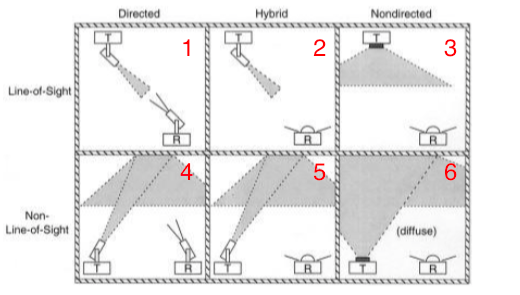
\includegraphics[width=7cm]{figuras/difuso}
		\caption{Transmissão na linha de visão e fora da linha de visão.}
		\label{fig:difuso}
\end{figure}

\end{frame}

\section{Hardware}
\begin{frame}{Montagem de Hardware}

Para realizar a comunicação VLC foi projetado um sistema com a seguinte especificação.

\begin{itemize}
	\item Comunicação ponto a ponto;
	\item Unidirecional;
	\item Canal aéreo.
\end{itemize}

\begin{figure}[!htb]
	\centering
		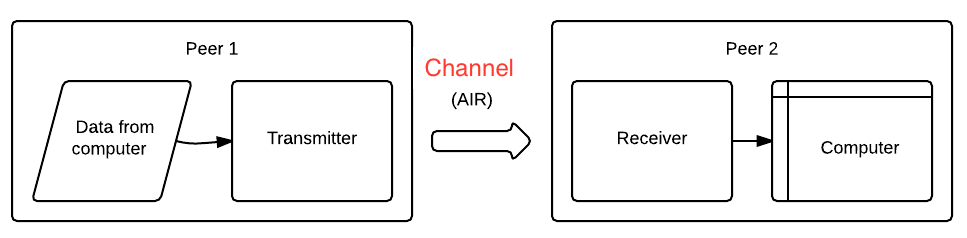
\includegraphics[width=7cm]{figuras/network-connection}
		\caption{Diagrama de transmissão ponto a ponto.}
		\label{fig:transmissao}
\end{figure}


\end{frame}

\begin{frame}{Montagem de Hardware}

\begin{itemize}
	\item Comunicação ponto a ponto;
	\item Unidirecional;
	\item Canal aéreo.
\end{itemize}

\begin{figure}[!htb]
	\centering
		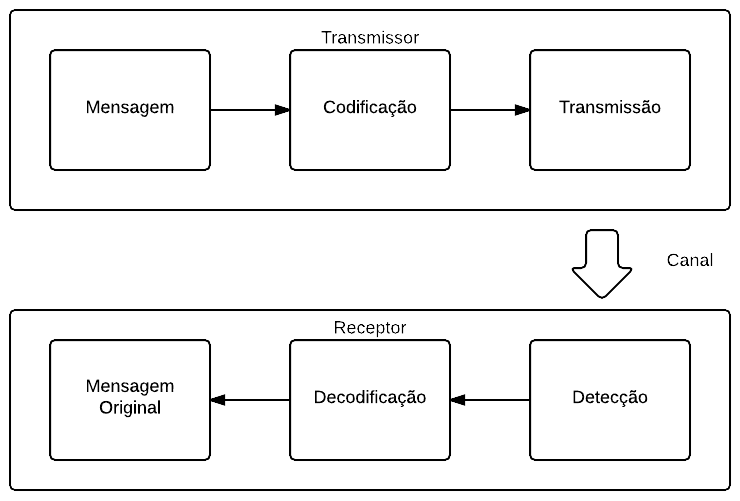
\includegraphics[width=7cm]{figuras/diagrama_transmissao}
		\caption{Diagrama de transmissão.}
		\label{fig:transmissao}
\end{figure}


\end{frame}


\subsection{Mensagem}
\begin{frame}{Codificação da Mensagem e Pacote}

A mensagem a ser enviada foi codificada utilizando a codificação OOK.

\begin{figure}[!htb]
	\centering
		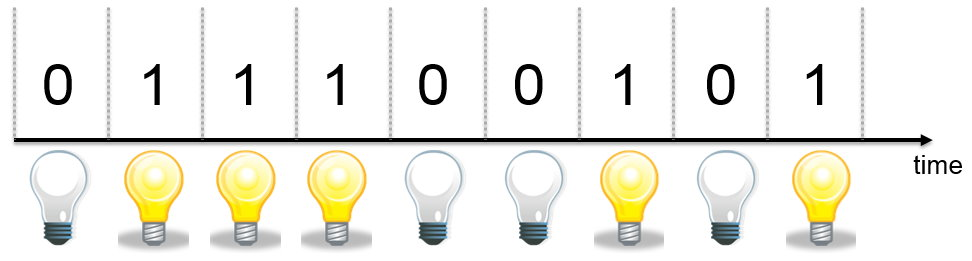
\includegraphics[width=7cm]{figuras/ook.jpg}
		\caption{Codificação de linha.}
		\label{fig:transmissao}
\end{figure}

\begin{figure}[!htb]
	\centering
		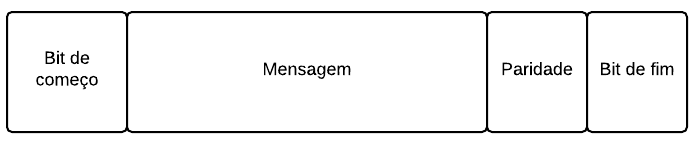
\includegraphics[width=7cm]{figuras/pacote}
		\caption{Organização do pacote.}
		\label{fig:transmissao}
\end{figure}


\end{frame}

\subsection{Transmissor}
\begin{frame}{Esquema de montagem transmissor}

Utiliza o microcontrolador MSP430 ligado a um LED que envia o pacote.

\begin{figure}[!htb]
	\centering
		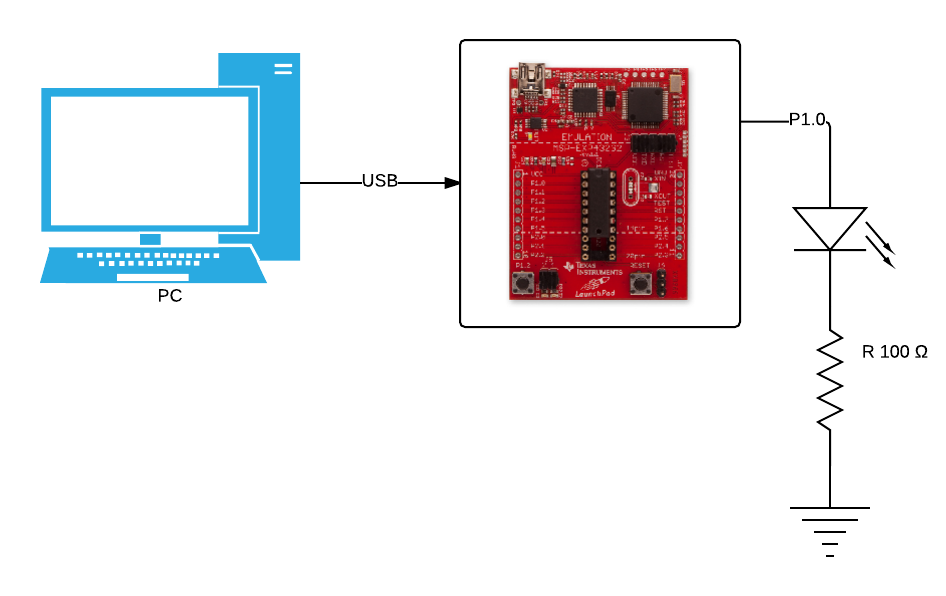
\includegraphics[width=7cm]{figuras/sistema-transmissao}
		\caption{Uso do controlador no Rx.}
		\label{fig:TX}
\end{figure}

\end{frame}



\begin{frame}{Uso do LED}

Os LEDs apresentam longa vida e baixo custo comparado as outras tecnologias de iluminação.

\begin{figure}[!htb]
	\centering
		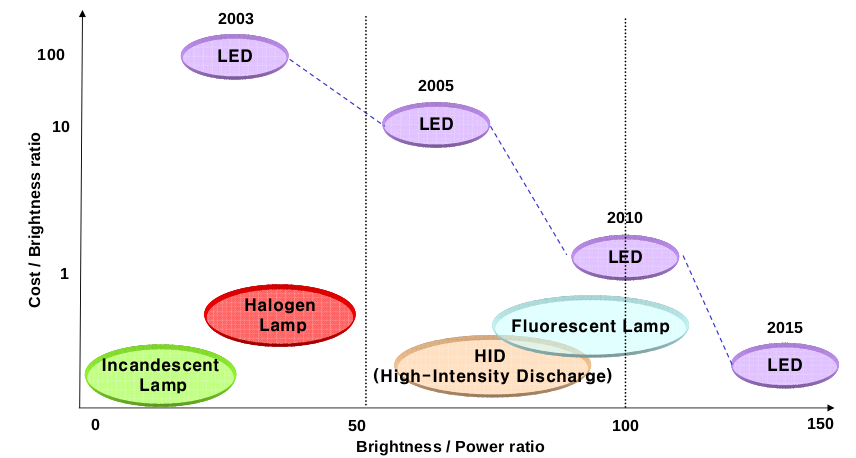
\includegraphics[width=7cm]{figuras/LED}
		\caption{O custo e eficiência do LED vem crescendo a cada dia.}
		\label{fig:custo led}
\end{figure}

\end{frame}


\subsection{Receptor}
\begin{frame}{Esquema de montagem transmissor}

Foi utilizado um conversor ADC para converter o sinal recebido em binário novamente.

\begin{figure}[!htb]
	\centering
		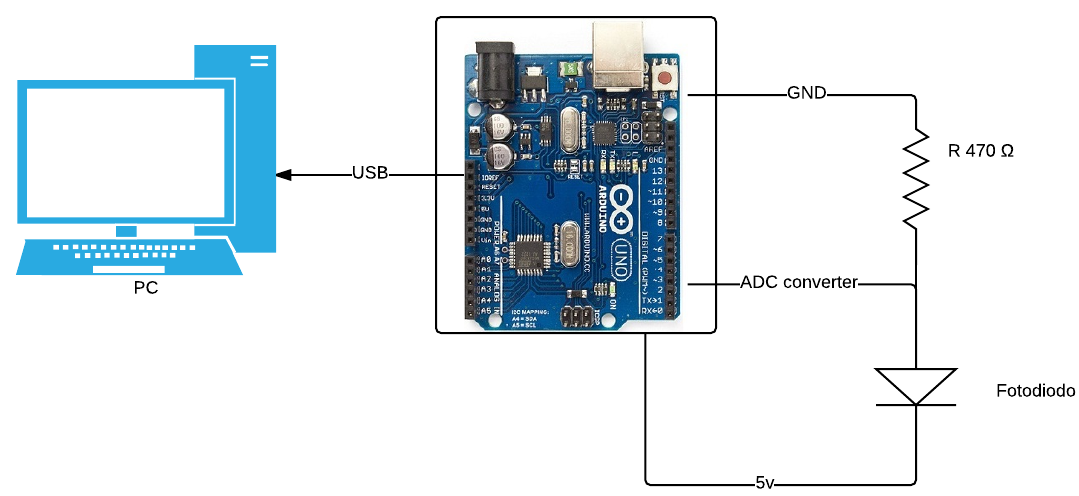
\includegraphics[width=7cm]{figuras/sistema_recepcao}
		\caption{Circuito utilizado para receber o sinal VLC.}
		\label{fig:Rx}
\end{figure}


\end{frame}


\begin{frame}{Características do Fotodiodo}

O fotodiodo utilizado possui ângulo de recepção baixo, dificultando a recepção se o conjunto estiver desalinhado.

\begin{figure}[!htb]
	\centering
		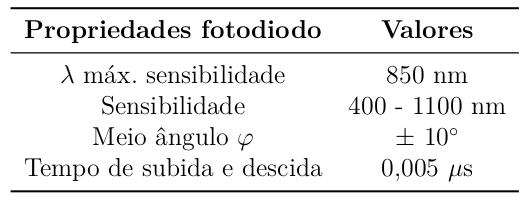
\includegraphics[width=7cm]{figuras/fotodiodo_chart}
		\caption{Especificações básicas do fotodiodo.}
		\label{fig:fotodiodo}
\end{figure}

\end{frame}

\section{Teste}
\begin{frame}{Teste de funcionalidade}

\begin{itemize}
\item Sensores ópticos alinhados;
\item Canal de comunicação aéreo;
\item Ambiente fechado Indoor;
\item Distância de 7.5 cm entre os sensores;
\item Iluminação ambiente;
\item Taxa de transmissão de 100 a 500 Hz.
\end{itemize}

\end{frame}

\begin{frame}{Hardware montado em protoboard}


\begin{figure}[!htb]
	\centering
		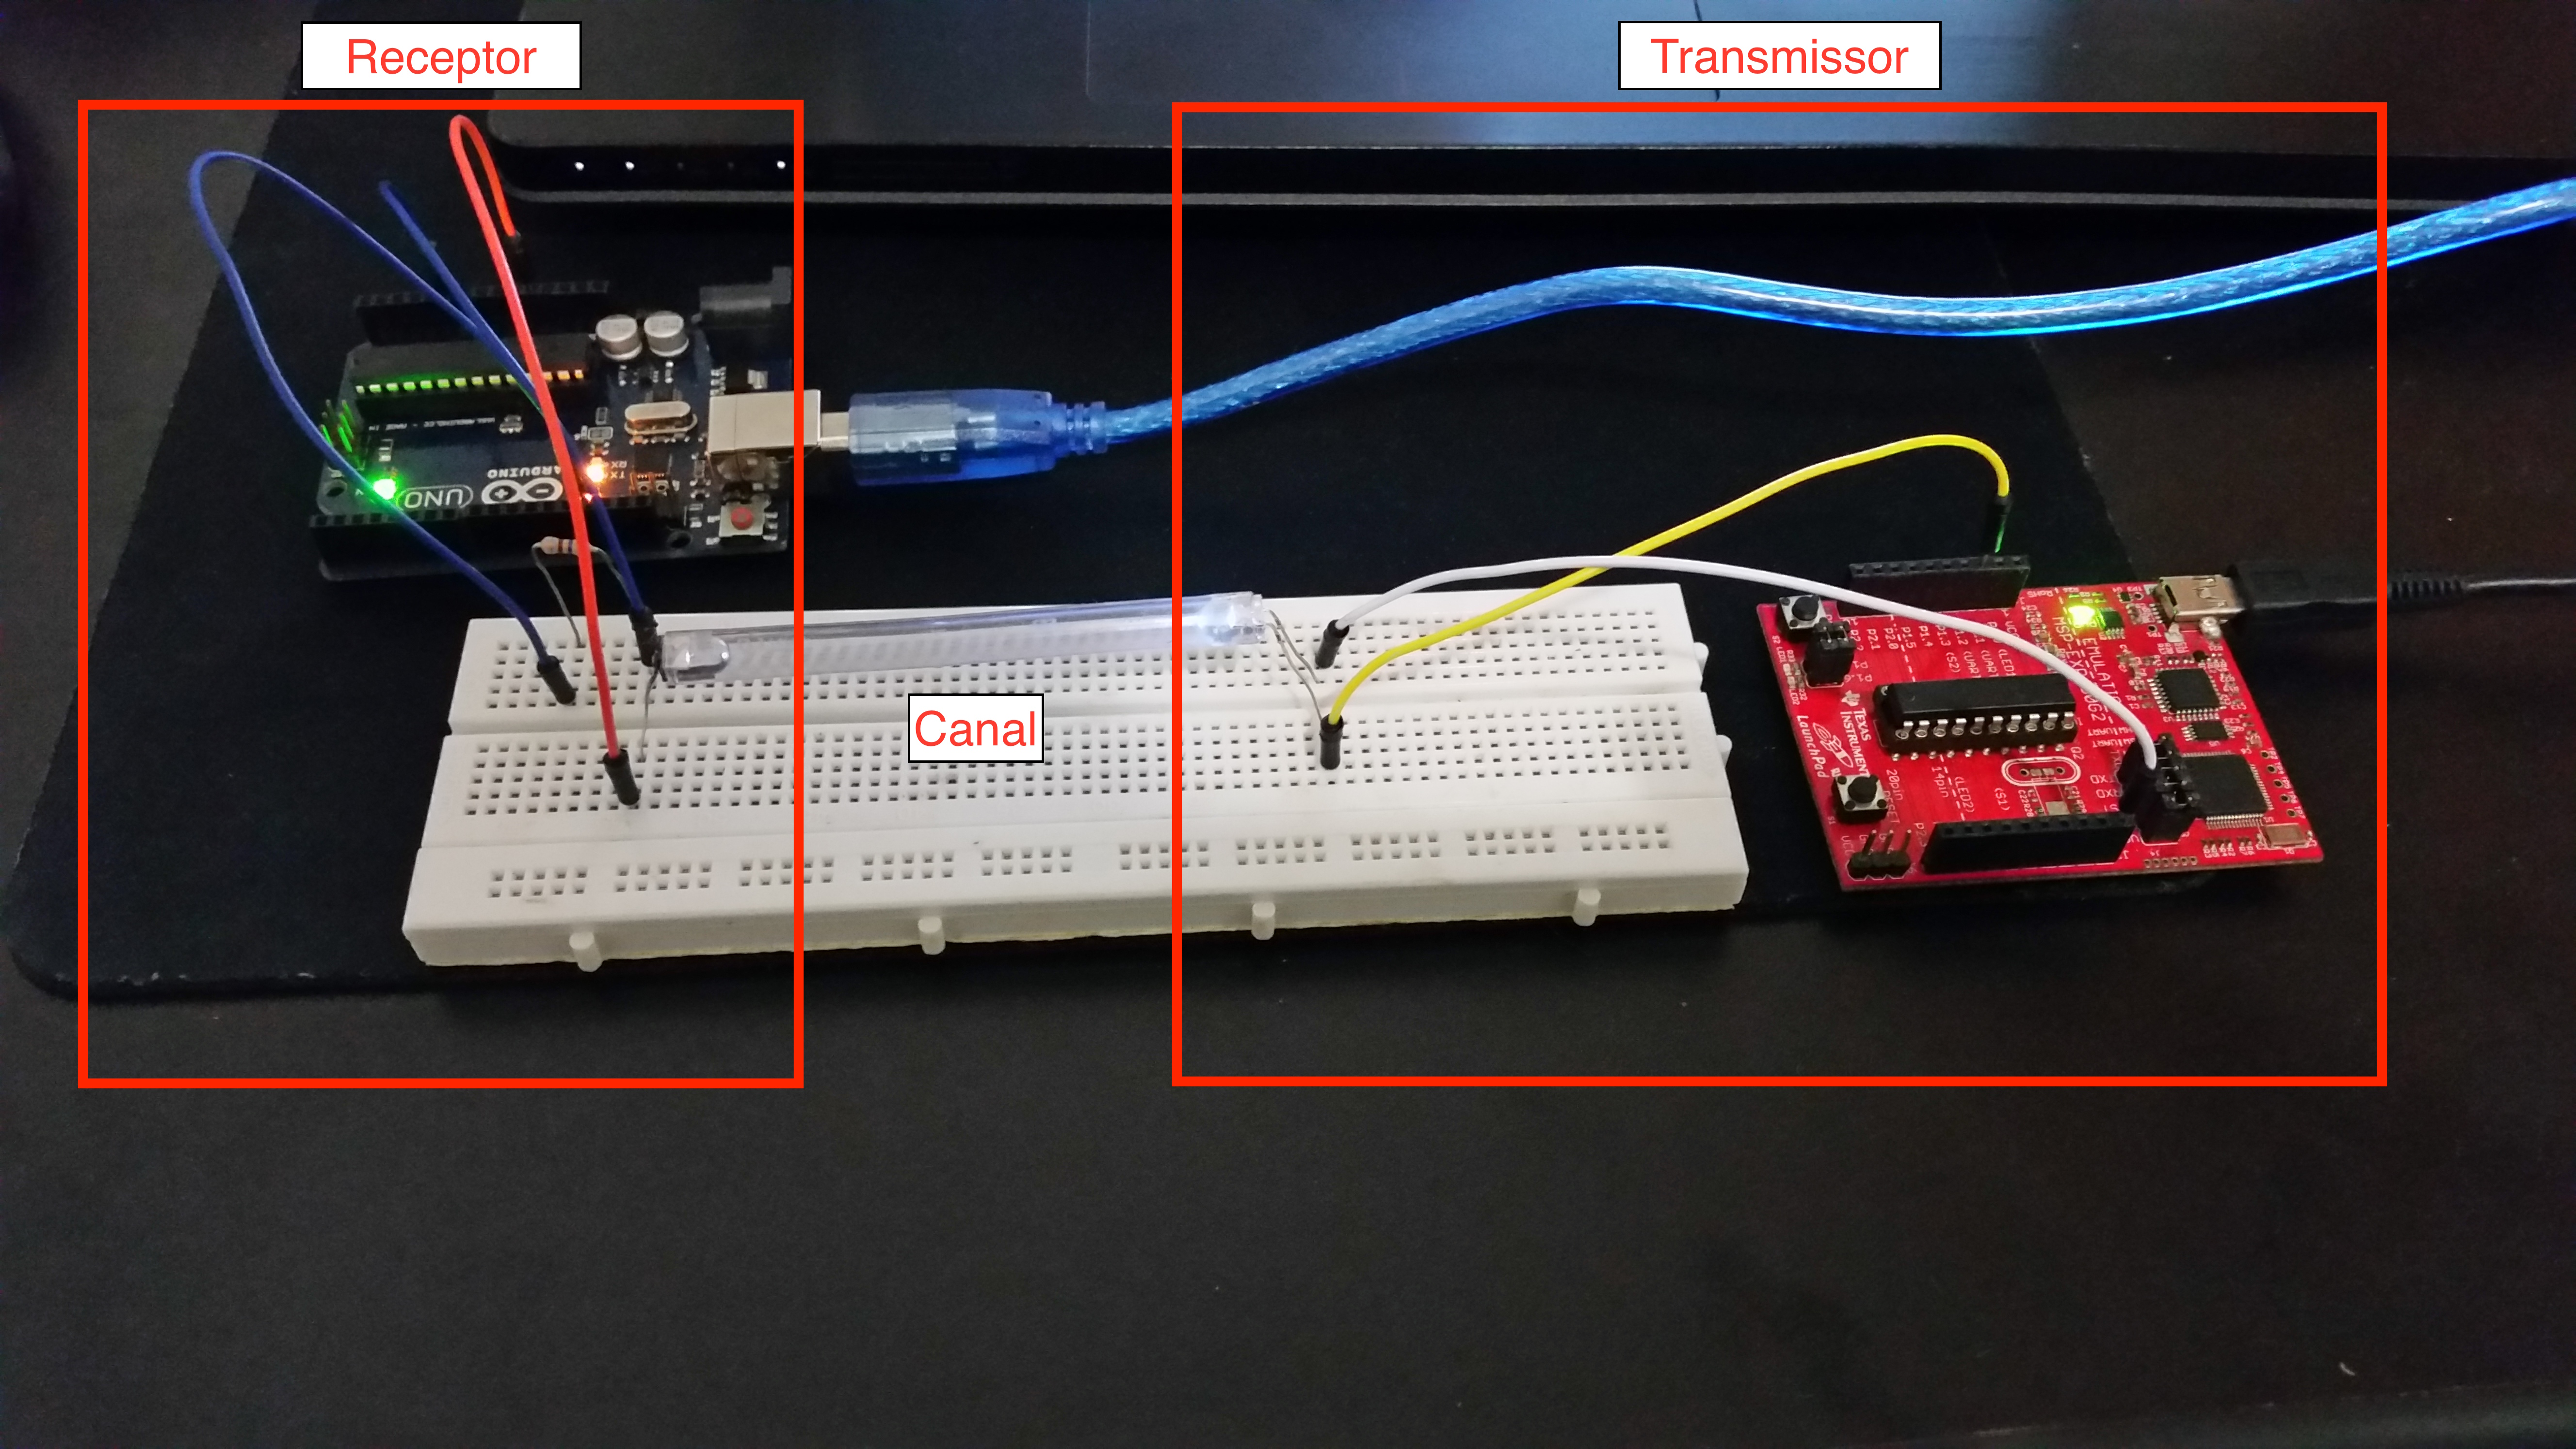
\includegraphics[width=7cm]{figuras/hardware}
		\caption{Foto do hardware montado.}
		\label{fig:montado}
\end{figure}

\end{frame}

\begin{frame}
Foi alta a taxa de erro para frequências acima de 400Hz.

\begin{figure}[!htb]
	\centering
		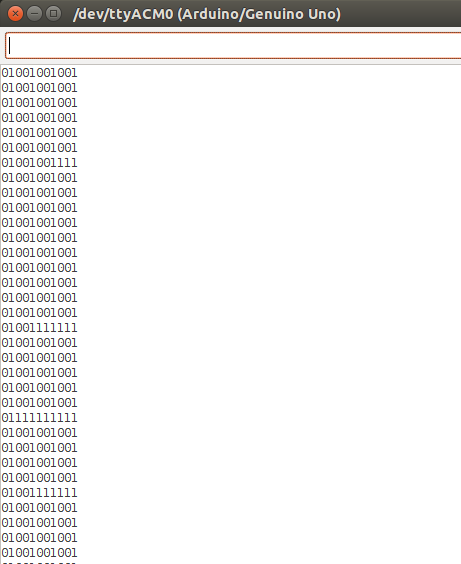
\includegraphics[width=7cm]{figuras/part5}
		\caption{Dados recebidos a 400Hz.}
		\label{fig:teste}
\end{figure}

\end{frame}

\begin{frame}{Conclusão}

\begin{itemize}
	\item O protótipo se mostrou funcional;
	\item Para frequências $<$ 300Hz erros nulos;
	\item Curto alcance;
	\item Forte interferências da iluminação ambiente;
	\item Atual configuração se mostra limitada.
\end{itemize}

\end{frame}

\section{Propostas Futuras}
\begin{frame}{Diagrama de envio de dados.}
Para aprimorar a transmissão de dados e ampliar a taxa de envio, é proposto um novo hardware com tais características.

\begin{figure}[!htb]
	\centering
		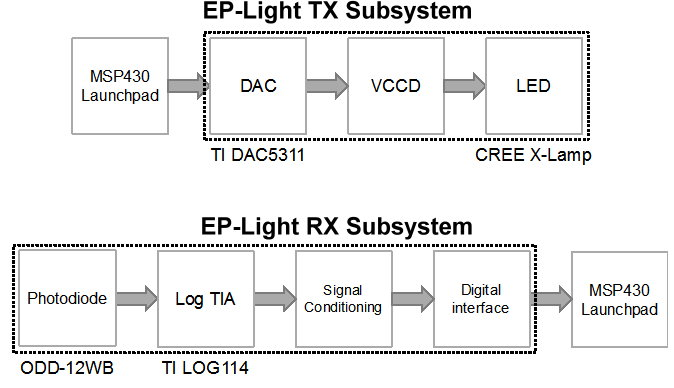
\includegraphics[width=7cm]{figuras/sistema-futuro-recptor}
		\caption{Sistema de transmissão futuro.}
		\label{fig:teste}
\end{figure}

\end{frame}



\begin{frame}{Cronograma do projeto}

\begin{figure}[!htb]
	\centering
		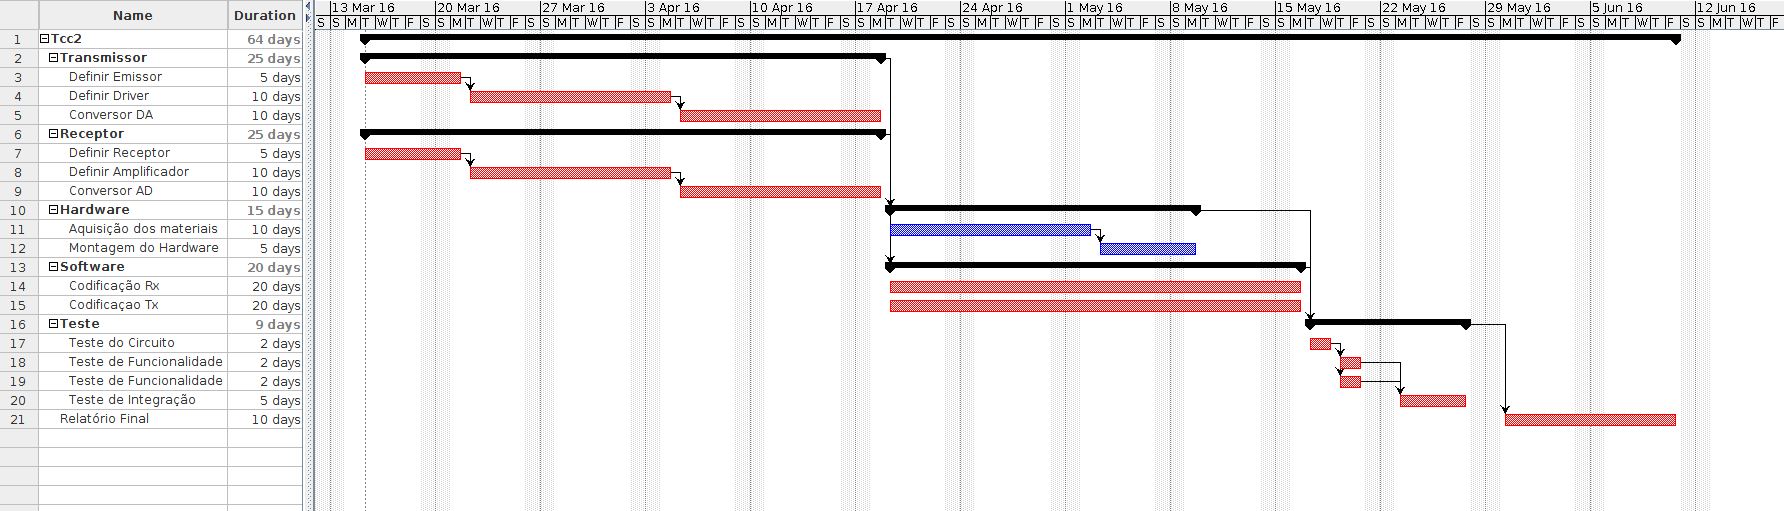
\includegraphics[width=11cm]{figuras/Grantt_diagram}
		\caption{Organização da segunda parte do projeto.}
		\label{fig:teste}
\end{figure}

\end{frame}


\begin{frame}{Diagrama de Fluxo}

\begin{figure}[!htb]
	\centering
		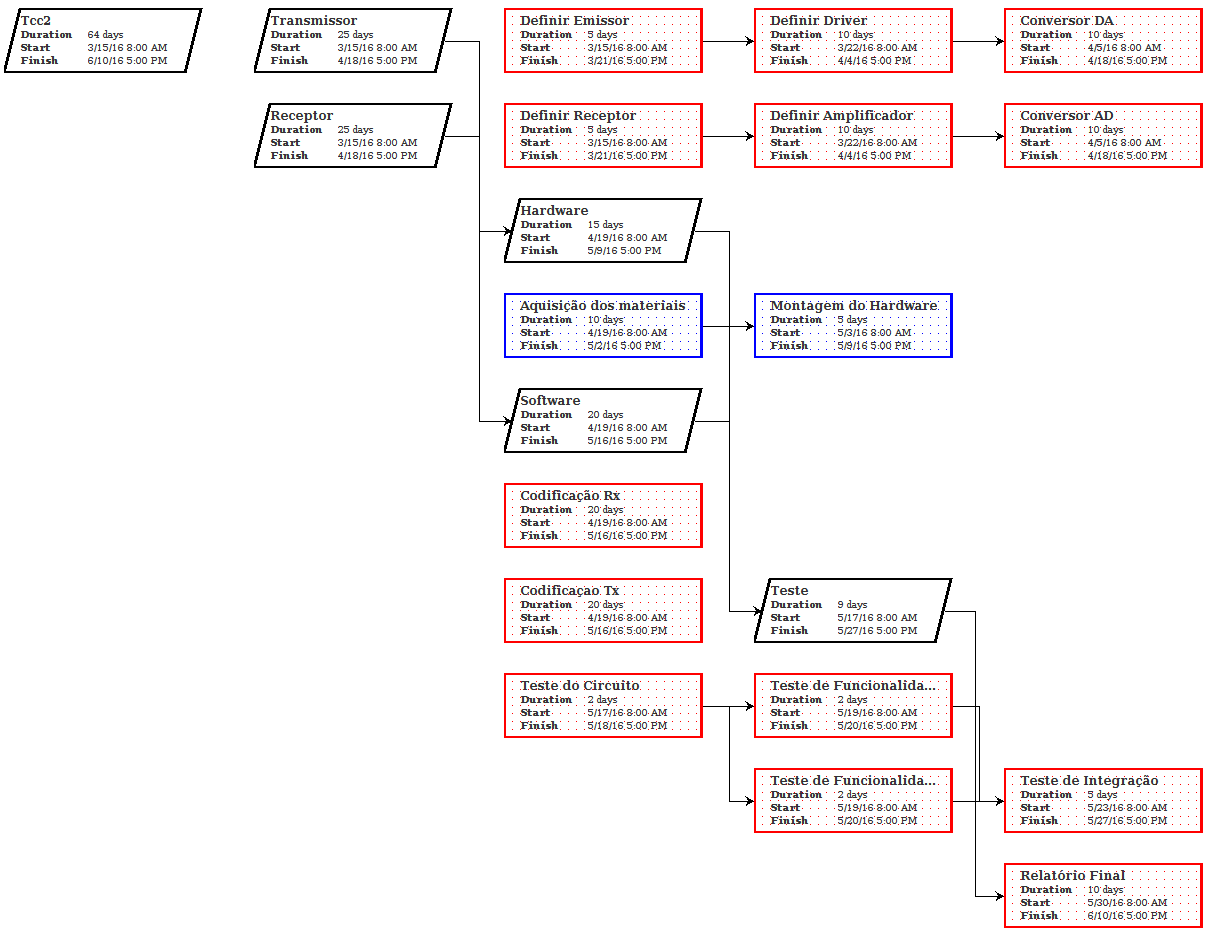
\includegraphics[width=8.5cm]{figuras/Network_diagram}
		\caption{Diagrama de dependências.}
		\label{fig:teste}
\end{figure}

\end{frame}

\end{document}

%\begin{multicols}{2}
%\end{multicols}


%\begin{figure}[!htb]
%\centering
%\includegraphics[width=7cm]{fig1}
%\caption{Code 1}
%\label{fig:Code 1}
%\end{figure}
